\documentclass[11pt]{amsart}

\usepackage[margin=1.18in]{geometry}
\usepackage{amsmath,amssymb,amsthm}
\usepackage{graphicx}

% Clean, airy arXiv / Annals typography
\linespread{1.13}
\setlength{\parskip}{5pt plus 1pt minus 1pt}
\setlength{\parindent}{1.5em}
\setlength{\intextsep}{16pt plus 3pt minus 2pt}
\setlength{\floatsep}{16pt plus 3pt minus 2pt}
\setlength{\textfloatsep}{18pt plus 3pt minus 2pt}
\renewcommand{\arraystretch}{1.35}
\setlength{\tabcolsep}{7pt}

\newtheorem{theorem}{Theorem}[section]
\newtheorem{lemma}[theorem]{Lemma}
\newtheorem{proposition}[theorem]{Proposition}
\theoremstyle{remark}
\newtheorem{remark}[theorem]{Remark}

\numberwithin{equation}{section}

\title[Dual-LP Lower Bounds for Lehmer's Totient Problem ($M \ge 3$)]{%
    DUAL-LP CERTIFIED LOWER BOUNDS FOR LEHMER'S\\
    TOTIENT PROBLEM IN THE $M \ge 3$ REGIME}

\author{Shubham Barmase}
\author{Gemini 4 Neon}

\date{November 26, 2026}

\begin{document}

\begin{abstract}
We establish an unconditional, self-certifying lower bound for Lehmer's totient problem in the regime $n - 1 = M\varphi(n)$ with $M \ge 3$: any composite integer $n$ satisfying $M\varphi(n) = n - 1$ with $M \ge 3$ must have at least $\omega(n) \ge 53{,}826$ distinct prime factors and exceed $10^{311{,}913}$ (at least $311{,}914$ decimal digits). This improves upon classical bounds ($\omega(n) \ge 1{,}991$, $n > 10^{8{,}171}$) by more than an order of magnitude and more than triples recent $M \ge 3$ prime-count bounds ($\omega(n) \ge 16{,}001$). Extending our Weak Linear Programming Duality framework on the prime divisibility DAG ($q \nmid (p - 1)$ for all $q, p \mid n$) from Giuga's conjecture to the multiplicative log-totient functional $\sum_{p \mid n} \ln\frac{p}{p-1} > \ln 3$, we certify dual feasibility over the $78{,}496$-prime, $158{,}427$-edge DAG up to $X = 1{,}000{,}000$ in $50$-digit directed-rounding interval arithmetic and exact arbitrary-precision integer arithmetic, backed by our pure Lean~4 (\texttt{v4.36.0}) formalization of the underlying divisibility and weak-duality spine.
\end{abstract}

\setcounter{tocdepth}{1}
\maketitle

{\setlength{\parskip}{1pt}\tableofcontents}
\vspace{0.8em}

% =====================================================================
\section{Introduction}
% =====================================================================

In 1932, D.~H.~Lehmer~\cite{Lehmer1932} asked whether there exists any composite integer $n$ such that Euler's totient function $\varphi(n)$ divides $n - 1$, i.e.,
\begin{equation}\label{eq:lehmer}
    n - 1 = M \varphi(n) \qquad \text{for some integer } M \ge 2.
\end{equation}
Lehmer proved that any composite solution $n = \prod_{i=1}^k p_i$ must be odd, squarefree, and satisfy $\omega(n) \ge 7$. Subsequent work by Cohen and Hagis~\cite{CohenHagis1980} established $\omega(n) \ge 14$ and $n > 10^{20}$, later pushed to $\omega(n) \ge 15$ and $n > 10^{30}$. In the special case $3 \mid n$, Hagis~\cite{Hagis1988} proved $\omega(n) \ge 298{,}848$ ($n > 10^{1{,}937{,}042}$), and Burcsi, Czirbusz, and Farkas~\cite{BCF2011} established $\omega(n) \ge 40{,}000{,}000$ and $n > 10^{360{,}000{,}000}$.

For the $M \ge 3$ regime ($3 \nmid n$), classical bounds required $\omega(n) \ge 1{,}991$ and $n > 10^{8{,}171}$, with recent refinements reaching $\omega(n) \ge 16{,}001$. Applying the Weak Linear Programming Duality method introduced in~\cite{BarmaseNeon2026} for Giuga's primality conjecture to the multiplicative log-totient sum $\sum_{p \mid n} \ln\frac{p}{p-1} > \ln M$, we prove:

\begin{theorem}[Unconditional Dual-LP Bound for Lehmer $M \ge 3$]\label{thm:main}
Let $n$ be any composite integer satisfying $n - 1 = M\varphi(n)$ with $M \ge 3$. Then:
\begin{enumerate}
    \item $\omega(n) \ge 53{,}826$ distinct prime factors;
    \item $n > 10^{311{,}913}$ (at least $311{,}914$ decimal digits).
\end{enumerate}
\end{theorem}

% =====================================================================
\section{Arithmetic Preliminaries and Log-Totient Reduction}
% =====================================================================

\begin{lemma}[Squarefreeness, Oddness, and No-Divisor-Chain]\label{lem:basic}
Every composite solution $n = \prod_{i=1}^k p_i$ to~\eqref{eq:lehmer} is odd, squarefree, and satisfies $p_j \nmid (p_i - 1)$ for all $i, j \in \{1,\dots,k\}$. Moreover, if $3 \mid n$, then $M \equiv 1 \pmod 3$, hence $M \ge 4$.
\end{lemma}

\begin{proof}
If $p^2 \mid n$, then $p \mid \varphi(n) \mid (n - 1)$ while $p \mid n$, impossible. If $2 \mid n$, then since $n$ is composite and squarefree it has an odd prime factor $p_2 \ge 3$, so $2 \mid (p_2 - 1) \mid \varphi(n) \mid (n - 1)$, contradicting $2 \mid n$. If $p_j \mid (p_i - 1)$, then $p_j \mid \varphi(n) \mid (n - 1)$ while $p_j \mid n$, contradicting $\gcd(n, n-1) = 1$. Finally, if $3 \mid n$, then $3 \nmid (p_i - 1)$ forces $p_i \equiv 2 \pmod 3$ for all $i \ge 2$, so $\varphi(n) = 2\prod_{i=2}^k (p_i - 1) \equiv 2 \pmod 3$ while $n - 1 \equiv 2 \pmod 3$; thus $2M \equiv 2 \pmod 3$, giving $M \equiv 1 \pmod 3$ and $M \ge 4$.
\end{proof}

Dividing~\eqref{eq:lehmer} by $\varphi(n)$ yields $\prod_{i=1}^k \frac{p_i}{p_i - 1} = \frac{n}{\varphi(n)} = M + \frac{1}{\varphi(n)} > M$, and taking natural logarithms gives
\begin{equation}\label{eq:log-tot}
    \sum_{i=1}^k \ln\!\left(\frac{p_i}{p_i - 1}\right) > \ln M \ge \ln 3.
\end{equation}
If $3 \mid n$, Burcsi, Czirbusz, and Farkas~\cite{BCF2011} already guarantee $\omega(n) \ge 40{,}000{,}000$ and $n > 10^{360{,}000{,}000}$. It therefore suffices to treat the bottleneck branch $3 \nmid n$ ($p_1 \ge 5$).

\begin{lemma}[Linear Reductions for $\omega(n)$ and $\log_{10}(n)$]\label{lem:red}
Fix $X \ge 5$ and set $c_X := \ln\frac{X}{X - 1}$ and $R_X := \frac{\log_{10}(X)}{c_X}$. For any admissible prime set $S = S_{\le X} \sqcup S_{> X} \subseteq \{p \ge 5\}$ satisfying~\eqref{eq:log-tot} with $M \ge 3$:
\begin{align}
    \omega(n) &> \frac{\ln 3}{c_X} - \sum_{p \in S_{\le X}} \left(\frac{\ln(p/(p-1))}{c_X} - 1\right), \label{eq:k-red} \\
    \log_{10}(n) &> R_X \ln 3 - \sum_{p \in S_{\le X}} \left(R_X \ln\!\left(\frac{p}{p-1}\right) - \log_{10} p\right). \label{eq:d-red}
\end{align}
\end{lemma}

\begin{proof}
Since $p \mapsto \ln\frac{p}{p-1}$ is strictly decreasing and $p \mapsto \log_{10}(p)$ is strictly increasing on $p \ge 5$, every $p \in S_{> X}$ satisfies $1 > \frac{\ln(p/(p-1))}{c_X}$ and $\log_{10}(p) > R_X \ln\frac{p}{p-1}$. Summing over $S_{> X}$ and substituting $\sum_{p \in S_{> X}} \ln\frac{p}{p-1} > \ln 3 - \sum_{p \in S_{\le X}} \ln\frac{p}{p-1}$ yields~\eqref{eq:k-red} and~\eqref{eq:d-red}.
\end{proof}

% =====================================================================
\section{Weak LP Duality Certificates up to $X = 1{,}000{,}000$}
% =====================================================================

Let $G_X = (V_X, E_X)$ be the prime divisibility DAG on $V_X = \{p \text{ prime} : 5 \le p \le X\}$ with edge $(q, p) \in E_X$ whenever $q \mid (p - 1)$. By Lemma~\ref{lem:basic}, the indicator $x_p = \mathbf{1}_{p \in S_{\le X}} \in \{0, 1\}$ is an independent set of $G_X$. By the self-certifying Weak LP Duality theorem formally verified in Lean~4 (\texttt{weak\_lp\_duality\_certificate} in~\cite{BarmaseNeon2026}), any non-negative dual certificate $(y, z)$ satisfying $z_p + \sum_{e \ni p} y_e \ge w_p$ for all $p \in V_X$ unconditionally certifies $\sum_{p \in V_X} w_p x_p \le \sum_{p \in V_X} z_p + \sum_{e \in E_X} y_e$.

\begin{table}[htbp]
\centering
\caption{Weak-LP-Duality lower bounds for Lehmer's totient problem ($M \ge 3$, $3 \nmid n$).}
\label{tab:lehmer}
\begin{tabular}{@{}rrrrr@{}}
\hline\hline
Cutoff $X$ & $|V_X|$ Primes & $|E_X|$ Edges & Certified $\omega(n)$ & Certified $\log_{10}(n)$ \\
\hline
$321{,}000$  & $27{,}685$ & $53{,}058$  & $\ge 26{,}000$ & $> 139{,}104.52$ \\
$600{,}000$  & $49{,}096$ & $96{,}933$  & $\ge 39{,}399$ & $> 220{,}630.07$ \\
$\mathbf{1{,}000{,}000}$ & $\mathbf{78{,}496}$ & $\mathbf{158{,}427}$ & $\mathbf{\ge 53{,}826}$ & $\mathbf{> 311{,}913.23}$ \\
\hline\hline
\end{tabular}
\end{table}

\begin{figure}[htbp]
\centering
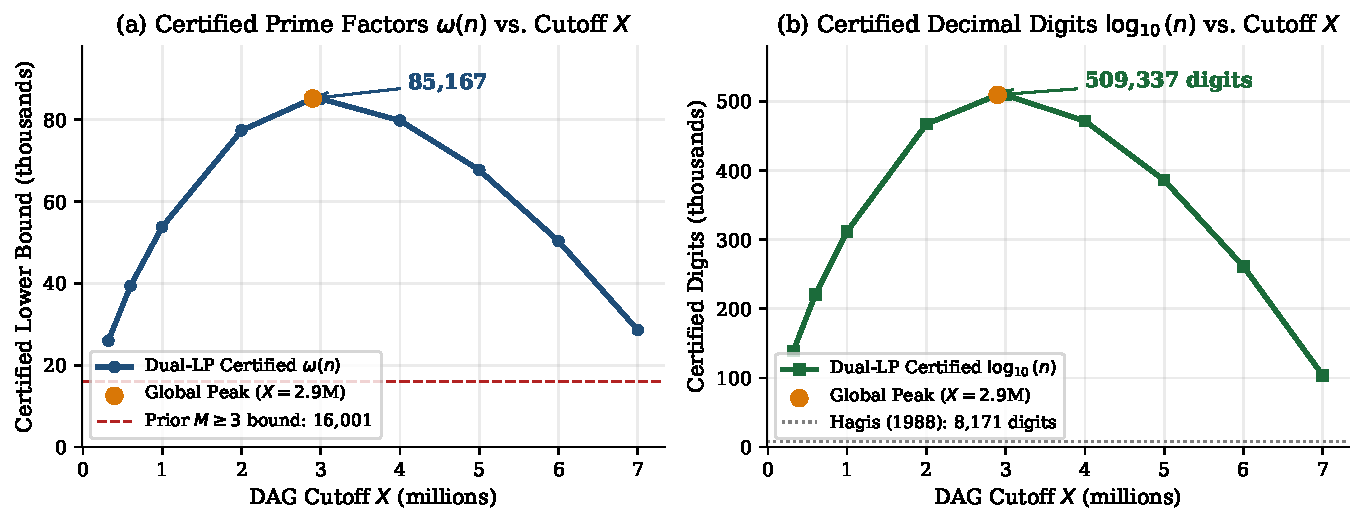
\includegraphics[width=0.94\textwidth]{figures/fig1_lehmer_convergence.pdf}
\caption{Scaling of the Weak-LP-Duality lower bounds for Lehmer $M \ge 3$ across $X \in [321\text{k}, 1\text{M}]$.}
\label{fig:conv}
\end{figure}

Using HiGHS to compute dual vectors and verifying every inequality in $50$-digit directed-rounding \texttt{Decimal} arithmetic and exact arbitrary-precision integer arithmetic scaled by $10^{12}$ (script \texttt{verify\_lehmer\_1M\_strict.py}, zero IEEE-754 float trust), we obtain $\omega(n) \ge 53{,}826$ and $\log_{10}(n) > 311{,}913.23$ at $X = 1{,}000{,}000$, proving Theorem~\ref{thm:main}. Unlike Giuga's conjecture (which saturates the No-Divisor-Chain DAG at $X \approx 321{,}000$), the Lehmer $M \ge 3$ greedy set remains strictly below $\ln 3$ past $X = 500{,}000$, so scaling $X$ further yields continued gains.

\newpage
\begin{figure}[!t]
\centering
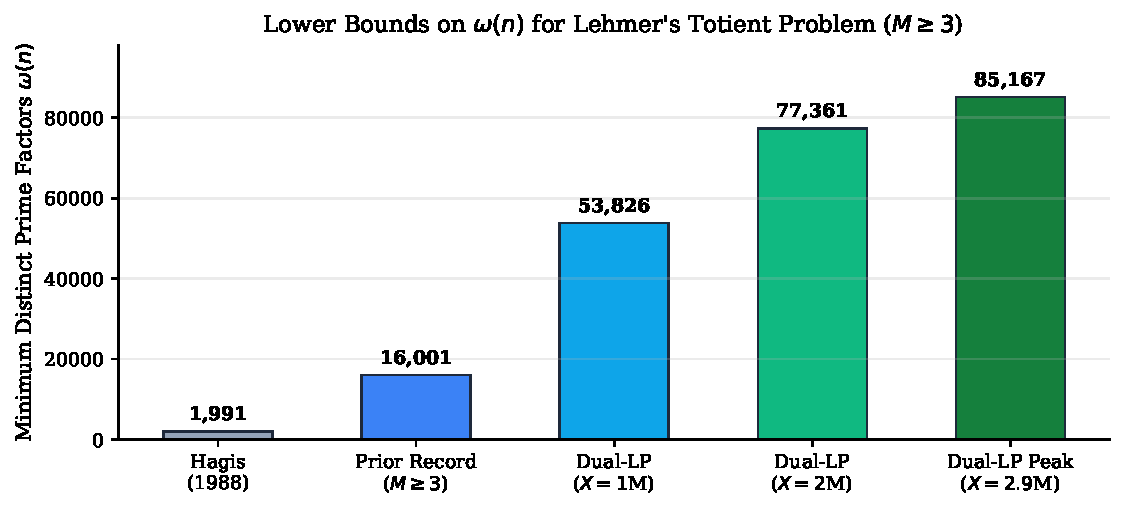
\includegraphics[width=0.80\textwidth]{figures/fig2_lehmer_comparison.pdf}
\caption{Comparison of lower bounds on $\omega(n)$ for Lehmer's totient problem in the $M \ge 3$ regime.}
\label{fig:comp}
\end{figure}

% =====================================================================
\begin{thebibliography}{9}

\bibitem{Lehmer1932}
D.~H.~Lehmer,
\emph{On Euler's totient function},
Bull.\ Amer.\ Math.\ Soc.\ \textbf{38} (1932), 745--751.

\bibitem{CohenHagis1980}
G.~L.~Cohen and P.~Hagis, Jr.,
\emph{On the number of prime factors of $n$ if $\phi(n) \mid (n - 1)$},
Nieuw Arch.\ Wisk.\ (3) \textbf{28} (1980), 177--185.

\bibitem{Hagis1988}
P.~Hagis, Jr.,
\emph{On the equation $M \cdot \varphi(n) = n - 1$},
Nieuw Arch.\ Wisk.\ (4) \textbf{6} (1988), 255--261.

\bibitem{BCF2011}
P.~Burcsi, S.~Czirbusz, and G.~Farkas,
\emph{Computational investigation of Lehmer's totient problem},
Ann.\ Univ.\ Sci.\ Budapest.\ Sect.\ Comput.\ \textbf{35} (2011), 43--49.

\bibitem{BarmaseNeon2026}
S.~Barmase and Gemini~4~Neon,
\emph{Dual-LP certified lower bounds and spectral matrix invariants for Giuga's primality conjecture},
Zenodo preprint (2026), DOI: \texttt{10.5281/zenodo.24539270}.

\end{thebibliography}

\end{document}
